\documentclass[11pt]{article}
%==============================================================================
%  Minimum-Fuel Low-Thrust GTO -> Cislunar Transfers:
%  Method, Regularization, and Lessons  (internal method note)
%
%  Source of record for numbers/claims:
%    GTO_tulip/process/LOW_THRUST_MINFUEL_CAMPAIGN.md
%    GTO_tulip/process/ROADMAP.md
%    GTO_ELFO/direct/elfo/ELFO_RETARGET.md
%==============================================================================
\usepackage[margin=1in]{geometry}
\usepackage{amsmath,amssymb,amsthm}
\usepackage{booktabs}
\usepackage{graphicx}
\usepackage{xcolor}
\usepackage{listings}
\usepackage[colorlinks=true,linkcolor=blue,citecolor=blue,urlcolor=blue]{hyperref}
\usepackage{enumitem}
\setlist{itemsep=2pt,topsep=3pt}
\emergencystretch=2.5em

% --- MATLAB code listing style ------------------------------------------------
\definecolor{codegray}{gray}{0.95}
\definecolor{codekw}{rgb}{0.13,0.13,0.7}
\definecolor{codecomment}{rgb}{0.0,0.5,0.0}
\definecolor{codestr}{rgb}{0.6,0.1,0.1}
\lstdefinestyle{mat}{
  language=Matlab, basicstyle=\ttfamily\footnotesize,
  keywordstyle=\color{codekw}, commentstyle=\color{codecomment}\itshape,
  stringstyle=\color{codestr}, backgroundcolor=\color{codegray},
  numbers=none, breaklines=true, frame=single, framerule=0pt,
  showstringspaces=false, columns=fullflexible, keepspaces=true, aboveskip=6pt, belowskip=6pt}
\lstset{style=mat}
\newcommand{\code}[1]{\texttt{\small #1}}
\newcommand{\file}[1]{\texttt{\small #1}}

% --- math shorthands ----------------------------------------------------------
\newcommand{\rv}{\mathbf{r}}
\newcommand{\vv}{\mathbf{v}}
\newcommand{\uv}{\boldsymbol{\alpha}}
\newcommand{\ND}{\mathrm{ND}}
\newcommand{\muS}{\mu^\star}
\newcommand{\dd}[2]{\frac{\mathrm{d}#1}{\mathrm{d}#2}}
\newcommand{\Tmax}{T_{\max}}
\newcommand{\rE}{r_1}
\newcommand{\rM}{r_2}
\DeclareMathOperator*{\argmin}{arg\,min}

\title{\bfseries Minimum-Fuel Low-Thrust GTO\,$\rightarrow$\,Cislunar Transfers\\[2pt]
       \large Method, Regularization, and Lessons\\[6pt]
       \normalsize (tulip and ELFO targets --- internal method note)}
\author{M.\ Casey}
\date{\today}

\begin{document}
\maketitle

\begin{abstract}
\noindent
We document the complete method used to compute certified minimum-fuel
low-thrust transfers from a geostationary transfer orbit (GTO) to two cislunar
destinations in the Earth--Moon circular restricted three-body problem (CR3BP):
a south-pole \emph{tulip} orbit and an elliptical lunar frozen orbit (ELFO).
The minimum-fuel problem is the hard member of the min-time / min-energy /
min-fuel trio because its cost is \emph{linear} in the throttle, so the optimum
is genuinely bang-bang (burn near perigee, coast near apogee) with dozens of
switches, and it lives on a $\sim$40-revolution spiral whose perigee passes
give catastrophic sensitivity. The working recipe is a three-stage pipeline:
(i) solve the min-\emph{time} problem as a robust root; (ii) generate
min-\emph{energy} seeds across a band of transfer times; and (iii) continue a
Bertrand--\'Ep\'enoy energy$\rightarrow$fuel homotopy at each transfer time.
Two regularizations make the collocation tractable: a Sundman change of
independent variable (single- and two-primary clocks) and the smooth-to-sharp
energy$\rightarrow$fuel deformation. We give the governing mathematics of each
stage, tie every step to the implementing MATLAB/CasADi code, and collect the
hard-won lessons --- chief among them that the exact NLP Hessian, an asset for a
well-scaled problem, \emph{destabilizes} near the gravitational singularities
unless the transcription is regularized first.
\end{abstract}

\tableofcontents

%==============================================================================
\section{Introduction and problem statement}\label{sec:intro}
%==============================================================================

\subsection{The transfer problem}
A low-thrust spacecraft departs a GTO ($350\times35\,786$~km, argument of
perigee $-25^\circ$) and must rendezvous with a cislunar science orbit. High
specific impulse ($I_{sp}=2100$~s) trades trip time for propellant, and for a
rideshare drop-off at GTO the propellant mass dominates the economics. We treat
two destinations, both specified as \emph{fixed rendezvous states} in the
rotating CR3BP frame:
\begin{itemize}
  \item the \textbf{tulip}: a south-pole-favorable petal orbit used for lunar
        south-pole navigation/relay geometry; and
  \item the \textbf{ELFO} (\code{im\_elfo\_optimum}: semi-major axis
        $12\,000$~km, eccentricity $0.69$, inclination $56.5^\circ$, argument of
        perilune $90^\circ$): an Intuitive-Machines-style data-relay reference.
\end{itemize}
Spacecraft and dynamics parameters are fixed throughout: initial mass $15$~kg,
maximum thrust $25$~mN, $I_{sp}=2100$~s, and Earth--Moon mass ratio
$\muS = 0.012150585609624$. All quantities are non-dimensional (ND): lengths in
units of the Earth--Moon distance, time such that the synodic mean motion is
unity.

\subsection{The insertion (rendezvous) points}\label{sec:insertion}
Both targets are periodic (or quasi-periodic) orbits, so ``arrival'' means
rendezvous with a specific \emph{phase} of the target orbit. The choice of
phase is a modeling decision that materially affects the transfer, and we make
it explicit (Appendix~A):
\begin{itemize}
  \item \textbf{tulip} --- the \emph{campaign} point, a slow, far-from-Moon
        phase (distance to Moon $\approx 28\,300$~km, ND speed $0.31$). It lies
        on the tulip orbit and is a gentle low-thrust capture state.
  \item \textbf{ELFO} --- the \emph{nearest}-insertion point, the ELFO phase
        closest in full state to the tulip terminal (distance to Moon
        $\approx 16\,800$~km, ND speed $0.39$), chosen so the target-continuation
        that manufactures the ELFO seed (Section~\ref{sec:energy}) stays
        well-conditioned.
\end{itemize}
Every result in this note is for these two insertion points; the pipeline is
target-agnostic, so retargeting to a different phase (e.g.\ the maximum-$\dot y$
tulip point or the ELFO apolune) is a one-line change followed by a re-solve.

\begin{figure}[htbp]
  \centering
  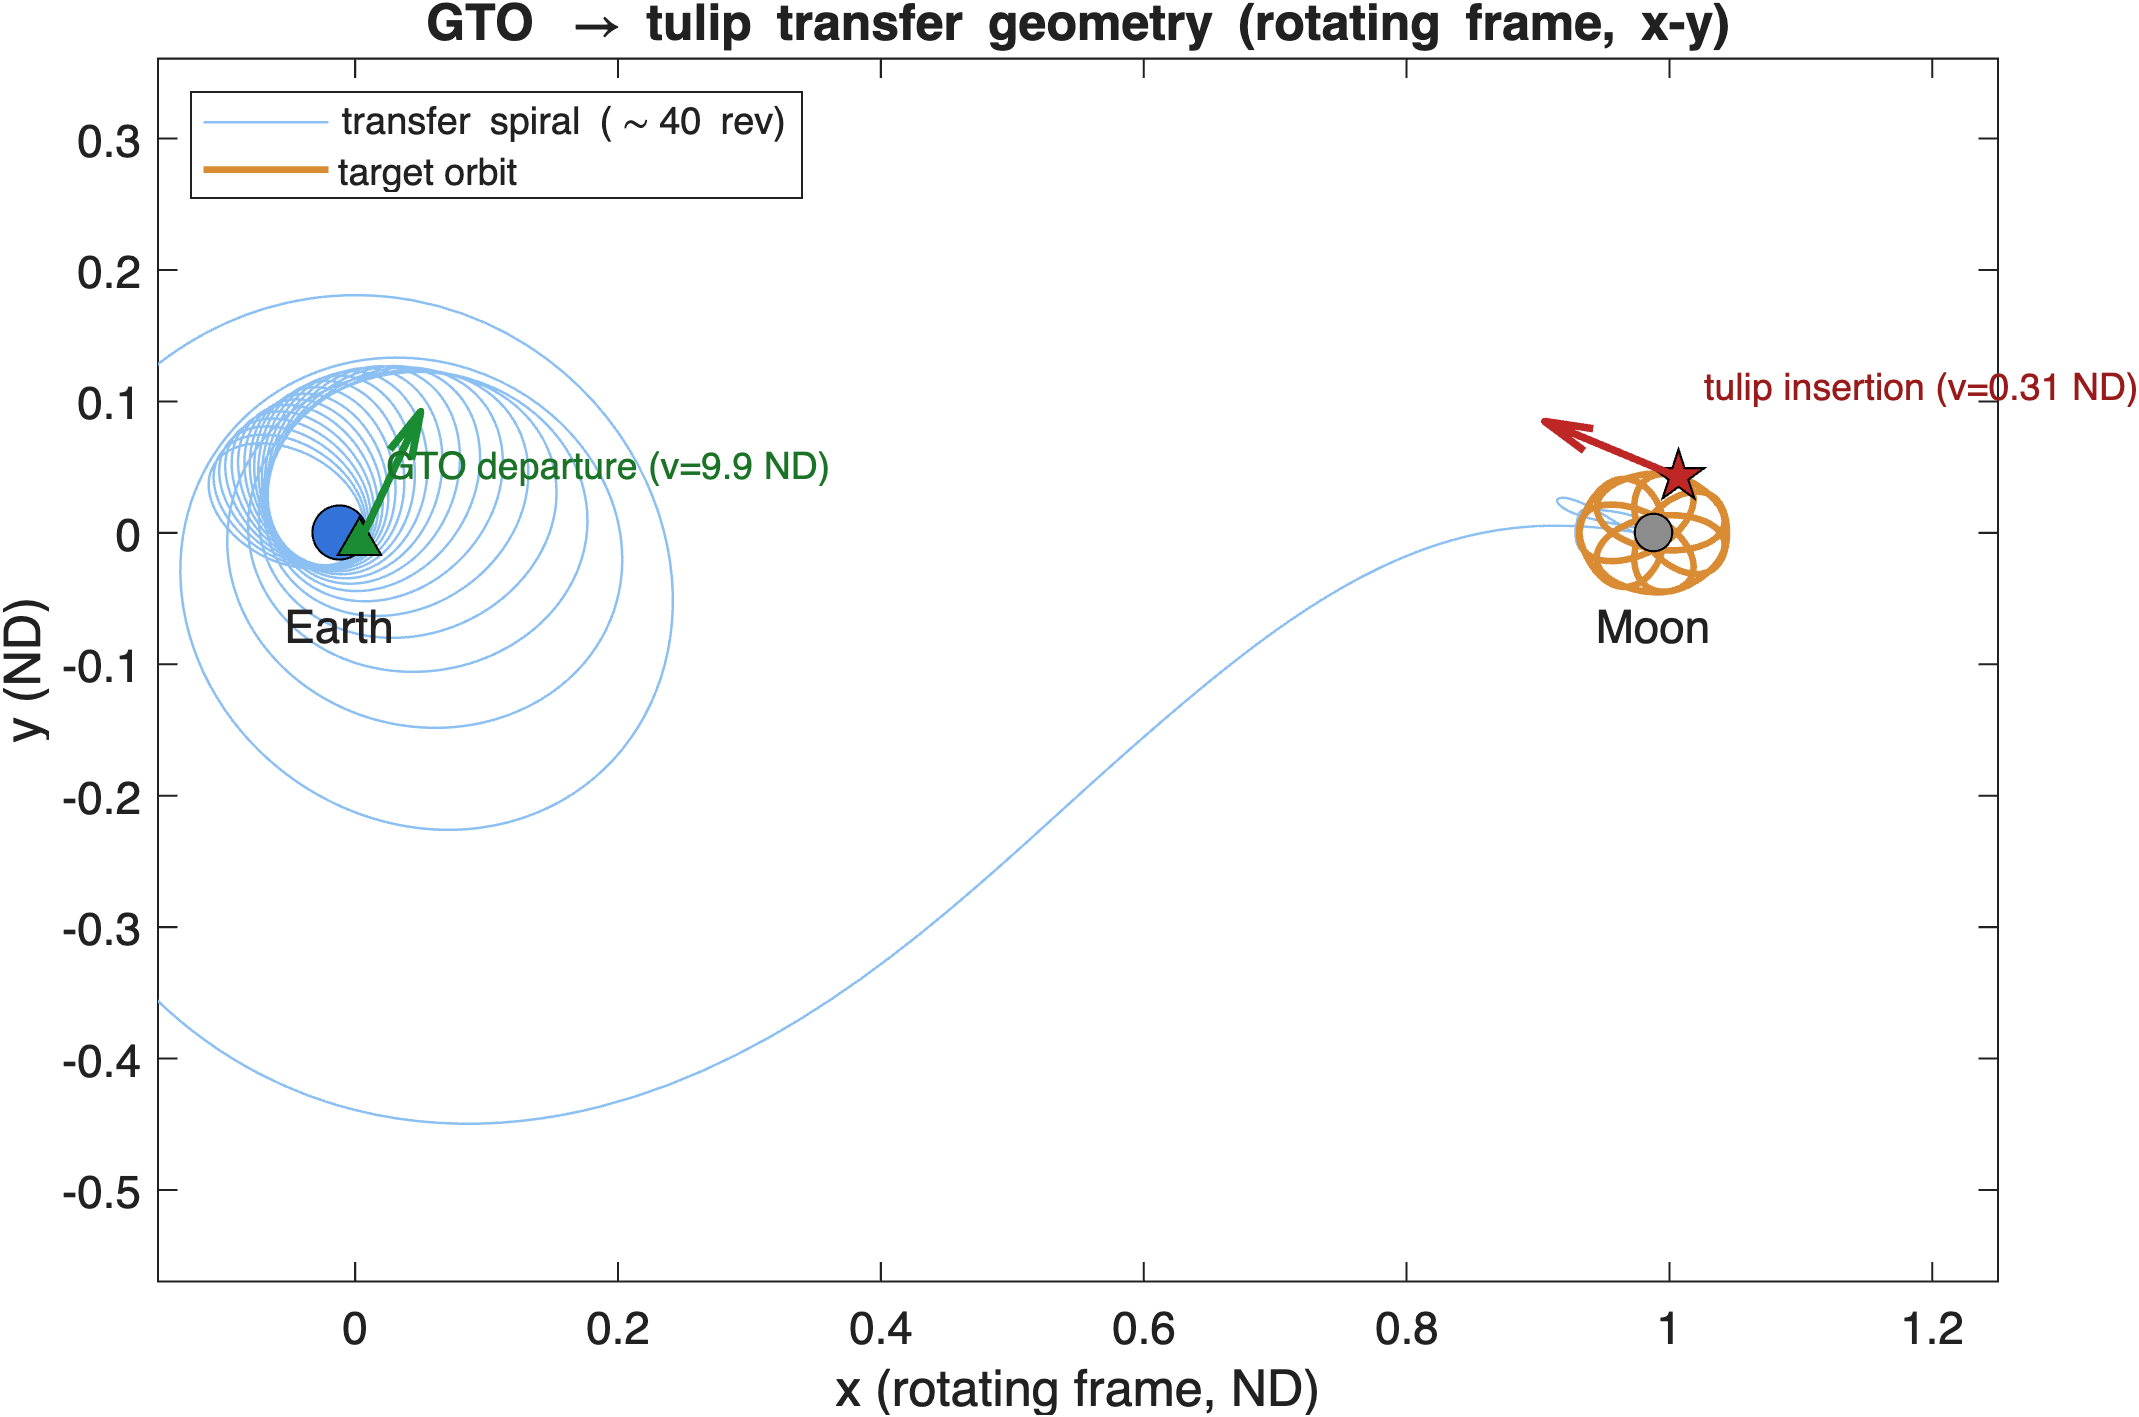
\includegraphics[width=0.82\textwidth]{figures/fig_geometry_tulip.png}
  \caption{GTO\,$\rightarrow$\,tulip transfer geometry in the rotating
    Earth--Moon frame. The $\sim$40-revolution transfer spiral (light blue)
    departs GTO near the Earth (green triangle, ND speed $9.9$) and rendezvous
    with the campaign insertion phase (red star, ND speed $0.31$) on the tulip
    orbit (orange) about the Moon. Arrows show the departure and insertion
    velocity directions.}
  \label{fig:geom-tulip}
\end{figure}

\subsection{Why minimum-fuel is the hard problem}\label{sec:why-hard}
Consider the three canonical objectives with running cost $L$, control throttle
$s\in[0,1]$, and thrust direction $\uv$, $\lVert\uv\rVert=1$:
\begin{equation}
  J_{\text{time}} = \!\int_0^{t_f}\! 1\,\mathrm{d}t,\quad
  J_{\text{energy}} = \!\int_0^{t_f}\! \tfrac12 s^2\,\mathrm{d}t,\quad
  J_{\text{fuel}} = \!\int_0^{t_f}\! s\,\mathrm{d}t .
\end{equation}
How the control enters $L$ decides everything, via Pontryagin's principle
(Section~\ref{sec:pmp}):
\begin{itemize}
  \item \textbf{Min-energy} is \emph{strictly convex} in $s$; the optimal
        control is the unique interior minimizer --- a \emph{continuous}
        saturated ramp. Smooth control $\Rightarrow$ smooth costate dynamics
        $\Rightarrow$ a large convergence basin. This is the genuinely easy
        problem, and it is our homotopy root.
  \item \textbf{Min-fuel} is \emph{linear} in $s$. Minimizing a linear function
        over a bounded set puts the optimum on a bound; the switching function
        crosses zero and the throttle jumps discontinuously --- genuine
        \emph{bang-bang} control.
  \item \textbf{Min-time} is bang-bang in principle, but for this transfer
        maximum thrust is always optimal (coasting only wastes time), so it
        \emph{degenerates} to always-on with \emph{no} interior switches. Its
        ease is problem-specific, not inherent smoothness.
\end{itemize}
Thus min-fuel is the only objective with genuine control discontinuities. That
non-smoothness (a) shrinks the indirect shooting basin to nothing and (b) makes
low-order collocation \emph{smear} the throttle, because a $0\!\to\!1$ jump
between two mesh nodes creates a large defect that the optimizer rounds off.

\paragraph{Two walls that compound.} The difficulty is really two independent
obstructions:
\begin{enumerate}
  \item \emph{Objective-side}: the bang-bang non-smoothness above.
  \item \emph{Dynamics-side}: the $\sim$40-revolution CR3BP spiral. Each of the
        $\sim$40 perigee passes contributes $\sim\!10^6$ shooting sensitivity,
        and the near-perigee $1/r^3$ gravity gradient destabilizes even an
        exact-Hessian Newton step. This wall is \emph{independent of the
        objective} --- min-time and min-energy face it too.
\end{enumerate}
Minimum-fuel is vicious precisely because it hands you \emph{both} walls at
once. The method of this note dismantles them separately: the
energy$\rightarrow$fuel homotopy removes wall~1 by starting from the convex
relaxation, and the Sundman regularization removes wall~2 by reparameterizing
the singular dynamics.

\subsection{Roadmap of the method}
The pipeline has three stages, developed in Sections~\ref{sec:mintime}--%
\ref{sec:homotopy} after the problem setup (Section~\ref{sec:ocp}) and the
Sundman regularization (Section~\ref{sec:sundman}) they all rely on:
\[
\underbrace{\text{min-time root}}_{\S\ref{sec:mintime}}
\;\longrightarrow\;
\underbrace{\text{min-energy seeds over a $t_f$ band}}_{\S\ref{sec:energy}}
\;\longrightarrow\;
\underbrace{\text{energy$\to$fuel homotopy per $t_f$}}_{\S\ref{sec:homotopy}} .
\]
Section~\ref{sec:verify} covers optimality verification, Section~\ref{sec:fronts}
the $\Delta V$--time fronts, and Section~\ref{sec:lessons} the transferable
lessons. Throughout, ``$\rightarrow$ \file{file.m}'' points at the implementing
code.

%==============================================================================
\section{The optimal control problem}\label{sec:ocp}
%==============================================================================

\subsection{CR3BP low-thrust dynamics}
In the rotating, barycentric, non-dimensional Earth--Moon frame the Earth sits
at $(-\muS,0,0)$ and the Moon at $(1-\muS,0,0)$. With position
$\rv=(x,y,z)$, velocity $\vv$, and mass $m$, define the distances to the
primaries
\begin{equation}
  \rE = \lVert \rv - (-\muS,0,0)\rVert,\qquad
  \rM = \lVert \rv - (1-\muS,0,0)\rVert .
\end{equation}
The controlled equations of motion are
\begin{align}
  \dot\rv &= \vv, \label{eq:rdot}\\
  \dot\vv &= \underbrace{\begin{pmatrix} x\\ y\\ 0\end{pmatrix}}_{\text{centrifugal}}
             + \underbrace{\begin{pmatrix} 2\dot y\\ -2\dot x\\ 0\end{pmatrix}}_{\text{Coriolis}}
             - (1-\muS)\frac{\rv-(-\muS,0,0)}{\rE^{3}}
             - \mu_g\,\muS\,\frac{\rv-(1-\muS,0,0)}{\rM^{3}}
             + \frac{s\,\Tmax}{m}\,\uv, \label{eq:vdot}\\
  \dot m  &= -\frac{\Tmax}{c}\,s, \label{eq:mdot}
\end{align}
where $c = I_{sp}\,g_0$ (ND exhaust velocity), $s\in[0,1]$ is the throttle,
$\uv$ is the unit thrust direction, and $\mu_g\in[0,1]$ is a
\emph{gravity-homotopy gain} on the Moon term only (Section~\ref{sec:energy});
$\mu_g\equiv1$ for the physical problem. Scaling only the Moon-gravity
coefficient --- and \emph{not} $\muS$ in the frame or Coriolis terms --- is
essential: touching $\muS$ elsewhere would move the barycenter and rotate the
frame underneath the boundary conditions.

\subsection{Control parameterization (cone elimination)}\label{sec:cone}
The thrust vector is $\mathbf{T} = s\,\Tmax\,\uv$ with $s\in[0,1]$ and
$\lVert\uv\rVert=1$. A na\"ive $(w_x,w_y,w_z)$ control with the cone constraint
$\mathbf{w}^\top\mathbf{w}=s^2$ is degenerate at coasts: as $s\to0$ the
direction $\mathbf{w}/\lVert\mathbf{w}\rVert$ becomes undefined, which wedges
the solver. We therefore carry the \emph{unit direction} $\uv$ and the
\emph{throttle} $s$ as separate decision variables with the single smooth
equality $\lVert\uv\rVert^2 = 1$; the direction stays well-defined through
coasts. $\rightarrow$ \file{casadi\_minfuel\_sundman.m}, \file{casadi\_energy\_freetf.m}.

\subsection{Boundary conditions}
With state $\mathbf{x}=(\rv,\vv,m)$, the transfer is a fixed-endpoint rendezvous:
\begin{equation}
  \rv(0),\vv(0) = \text{GTO departure } \rv_0,\qquad m(0)=1,\qquad
  \rv(t_f),\vv(t_f) = \text{insertion state } \rv_f,
\end{equation}
with final mass free. The endpoints $\rv_0,\rv_f$ come from a single explicit
source (Appendix~A); $\rv_0$ is common to both targets,
$\rv_f$ is the target's chosen insertion phase (Section~\ref{sec:insertion}).

\subsection{Pontryagin structure and the switching function}\label{sec:pmp}
Introduce costates $(\boldsymbol\lambda_r,\boldsymbol\lambda_v,\lambda_m)$ and
the Hamiltonian for the fuel problem,
\begin{equation}
  H = s\;+\;\boldsymbol\lambda_r^\top\vv
    \;+\;\boldsymbol\lambda_v^\top\!\Big(\mathbf{g}(\rv,\vv)+\tfrac{s\Tmax}{m}\uv\Big)
    \;-\;\lambda_m\tfrac{\Tmax}{c}s ,
\end{equation}
with $\mathbf{g}$ the ballistic (gravity + frame) acceleration. Minimizing $H$
over $\uv$ with $\lVert\uv\rVert=1$ gives the \emph{primer-vector} law
\begin{equation}
  \uv^\star = -\,\frac{\boldsymbol\lambda_v}{\lVert\boldsymbol\lambda_v\rVert},
  \label{eq:primer}
\end{equation}
i.e.\ thrust opposes the velocity costate. Substituting, $H$ is linear in $s$
with coefficient the \emph{switching function}
\begin{equation}
  S \;=\; 1 \;-\; \frac{\Tmax}{m}\lVert\boldsymbol\lambda_v\rVert
        \;-\; \frac{\Tmax}{c}\lambda_m ,
  \label{eq:switch}
\end{equation}
so the fuel-optimal throttle is bang-bang,
\begin{equation}
  s^\star = \begin{cases} 1 & S<0 \ (\text{burn}),\\[2pt]
                          0 & S>0 \ (\text{coast}),\end{cases}
  \label{eq:bangbang}
\end{equation}
with singular arcs only where $S\equiv0$ on an interval (not encountered here).
Equations~\eqref{eq:primer}--\eqref{eq:bangbang} are the first-order optimality
conditions we later verify against the direct solution's KKT multipliers
(Section~\ref{sec:verify}). The energy problem replaces the cost integrand
$s$ by $\tfrac12 s^2$, making $H$ \emph{strictly convex} in $s$ with the smooth
interior/clamped minimizer $s^\star=\mathrm{sat}_{[0,1]}\!\big(-S_e\big)$ for the
corresponding (shifted) switching function $S_e$ --- the continuous ramp that
makes energy well-conditioned.
%==============================================================================
\section{Sundman regularization}\label{sec:sundman}
%==============================================================================
All three objectives share the dynamics-side wall (Section~\ref{sec:why-hard}):
$\sim$40 perigee passes at $\rE\approx0.017$~ND (a $350$~km altitude), where the
gravitational curvature is enormous. We tame it by changing the independent
variable.

\subsection{The single-primary clock}\label{sec:sundman-single}
Replace physical time $t$ by a regularizing variable $\tau$ through the Sundman
relation
\begin{equation}
  \dd{t}{\tau} = \kappa(\rv),\qquad \kappa = \rE^{\,p},\quad p=1.5,
  \label{eq:sundman}
\end{equation}
and carry time as an extra state. Every equation of motion is multiplied by
$\kappa$: $\mathrm{d}\mathbf{x}/\mathrm{d}\tau = \kappa\,\mathbf{f}(\mathbf{x},u)$
with $\mathbf{f}$ the right-hand side of \eqref{eq:rdot}--\eqref{eq:mdot}. Two
benefits follow.

\paragraph{(i) Curvature reduction (not elimination).} Near the Earth the
ballistic acceleration scales as $\rE^{-2}$; multiplied by $\kappa=\rE^{\,p}$ it
becomes $\rE^{\,p-2}$. Its position Jacobian (the sensitivity carried by the
state-transition matrix) then scales as $\rE^{\,p-3}$, and its second derivative
--- the term that enters IPOPT's \emph{exact} Lagrangian Hessian --- as
$\rE^{\,p-4}$:
\begin{equation}
  \underbrace{\rE^{-2}}_{\text{accel}} \xrightarrow{\times\kappa} \rE^{\,p-2},
  \qquad
  \underbrace{\rE^{-4}}_{\text{accel Hessian}} \xrightarrow{\times\kappa}
  \rE^{\,p-4}.
  \label{eq:hessian-scaling}
\end{equation}
Sundman thus lowers every gravitational singular exponent by $p$. At $p=1.5$ the
acceleration Hessian goes from $\rE^{-4}$ to $\rE^{-2.5}$ --- a reduction of
$\rE^{\,p}\approx 0.017^{1.5}\approx 2\times10^{-3}$ (a factor of $\sim\!450$) at
the perigee. This is decisive, but note carefully that $\rE^{-2.5}\approx
2.6\times10^{5}$ is \emph{still large}: the regularization \textbf{tames but does
not eliminate} the singular curvature. That residual is exactly why (a) a
\emph{uniform} $\tau$-mesh is essential (next), and (b) the exact Hessian can
still destabilize near a primary, which forces the two-primary clock of
Section~\ref{sec:sundman-two} and underlies the ``exact-Hessian-hurts'' lesson
(Section~\ref{sec:lessons}). (The shorthand ``the $1/r^3$ Hessian becomes
bounded'' overstates the effect; \eqref{eq:hessian-scaling} is the precise
statement.)

\paragraph{(ii) Automatic node concentration.} Because
$\mathrm{d}\tau=\mathrm{d}t/\kappa=\mathrm{d}t/\rE^{\,p}$, a \emph{uniform} step
in $\tau$ spans a \emph{short} step in $t$ where $\rE$ is small. A uniform
$\tau$-mesh therefore concentrates collocation nodes near perigee in physical
time --- for free, without an $hp$-adaptive scheme --- exactly where the sharp
throttle switches and the largest defects live.

\subsection{The two-primary clock}\label{sec:sundman-two}
The single-primary clock $\kappa=\rE^{\,p}$ tames only the \emph{Earth} perigee.
For a Moon-vicinity target (both the tulip campaign point and the ELFO), the
terminal arc approaches the Moon, where the \emph{lunar} gravity Hessian
($\sim\rM^{-4}$) is left completely unregularized. Empirically this is fatal:
running the exact-Hessian min-time solve to the tulip with the single-primary
clock \emph{deterministically} overflows the near-Moon Hessian and crashes the
MUMPS factorization (Section~\ref{sec:mintime}). The cure is a smooth
\emph{min-distance} clock that regularizes both primaries,
\begin{equation}
  \kappa \;=\; \big(\rE^{-q} + (\rM/D)^{-q}\big)^{-p/q},
  \qquad q\approx4,\ D\approx0.15\ (\text{lunar SOI}),
  \label{eq:twoclock}
\end{equation}
which recovers $\kappa\to\rE^{\,p}$ near the Earth ($\rE\ll\rM$) and
$\kappa\to(\rM/D)^{\,p}$ near the Moon ($\rM\ll\rE$); $q$ sets the transition
sharpness and $D$ the crossover radius. Setting $D\le0$ recovers the
single-primary clock. The two-primary clock lowers \emph{both} singular
exponents by $p$ and redistributes nodes into the lunar-capture arc.
$\rightarrow$ \file{casadi\_energy\_freetf.m}, \file{casadi\_mintime\_freetf.m}.

\subsection{Free final time via a slack state}\label{sec:sundman-cscale}
The total regularized length $\tau_f$ is held \emph{fixed} (a numerical choice
tied to the warm start): a \emph{free} scalar $\tau_f$ would multiply every
collocation defect, producing one dense KKT column and catastrophic MUMPS
fill-in at large $N$. To let the physical transfer time $t_f$ vary anyway, we use
Betts' sparse free-time trick --- a constant slack \emph{state} $c$ (\code{cScale}):
\begin{equation}
  \dd{t}{\tau} = c\,\kappa(\rv),\qquad \dd{c}{\tau} = 0 .
  \label{eq:cscale}
\end{equation}
$c$ is one number, tied across nodes by \emph{local} continuity constraints, so
the Jacobian stays banded; $t_f=t(\tau_f)$ becomes a free outcome. Two subtleties
are worth stating precisely, as both are easy to get wrong:
\begin{itemize}
  \item \textbf{Min-energy needs a pinned $t_f$.} Free-$t_f$ minimum energy is
        ill-posed: the energy optimum always drifts to longer time (thinner
        thrust lowers $\int s^2\,\mathrm{d}t$), so IPOPT wanders off the warm
        start. We therefore \emph{pin} $t_f$ with a terminal constraint
        $t(\tau_f)=t_f^{\text{target}}$ and let $c$ float to satisfy it. The
        slack is not there to free $t_f$ for the energy solve; it holds a fixed
        $t_f$ cleanly under a \emph{changing} clock during continuation
        (Section~\ref{sec:energy}).
  \item \textbf{What the slack actually buys.} Its real benefit is
        \emph{decoupling} the trajectory shape from the $t_f/\tau_f$ ratio. The
        older fixed-$t_f$ single-primary solver
        (\file{casadi\_minfuel\_sundman.m}) has no slack: it fixes $\tau_f$ and
        pins $t(\tau_f)=t_f$ directly, so the constraint
        $\int_0^{\tau_f}\!\kappa\,\mathrm{d}\tau=t_f$ couples the trajectory
        geometry (through $\kappa=\rE^{\,p}$) to the scalar $t_f$. That coupling
        is benign for a single solve at the warm start's own $t_f$, but it
        stiffens badly under $t_f$-continuation --- which is why the free-time
        formulation \eqref{eq:cscale} superseded it.
\end{itemize}
The state and control layout is then
\begin{equation}
  \mathbf{x} = (\rv,\vv,m,t,c)\in\mathbb{R}^9,\qquad
  u = (\uv,s)\in\mathbb{R}^4,\ \lVert\uv\rVert=1,\ s\in[0,1].
\end{equation}

\subsection{Discretization}\label{sec:disc}
We use trapezoidal collocation on a normalized mesh $\sigma\in[0,1]$ with
$\tau=\sigma\,\tau_f$, so $\mathrm{d}\mathbf{x}/\mathrm{d}\sigma =
\tau_f\,\mathrm{d}\mathbf{x}/\mathrm{d}\tau$. With $F=c\,\kappa\,[\vv;\dot\vv;
\dot m;1]$ (the $\tau$-derivative) and nodes $k=0,\dots,N$, the defects and unit
constraint are
\begin{equation}
  \mathbf{D}_k = \mathbf{x}_{k+1}-\mathbf{x}_k
    - \tfrac{\tau_f\,\Delta\sigma_k}{2}\big(F_k+F_{k+1}\big) = \mathbf{0},
  \qquad \lVert\uv_k\rVert^2 - 1 = 0 .
  \label{eq:trap}
\end{equation}
The full NLP is assembled and differentiated automatically by CasADi (exact
sparse Jacobian and Hessian) and solved by IPOPT with the MUMPS linear solver.
The heart of the transcription is compact:
\begin{lstlisting}
% two-primary min-distance clock (moonZone<=0 -> single-primary r1^p)
if moonZone > 0
    kappa = ( r1^(-qSund) + (r2/moonZone)^(-qSund) )^(-pSund/qSund);
else
    kappa = r1^pSund;
end
% free physical time via the slack state cs:  dt/dtau = cs*kappa
fdyn = Function('f',{x,u},{[ cs*kappa*[v; accel; mdot; 1]; 0 ]});  % dX/dtau
% trapezoidal defects in sigma:  dX/dsigma = tauf*dX/dtau
D = X(:,2:end)-X(:,1:end-1) - tauf*(repmat(dsig,9,1)/2).*(F(:,1:end-1)+F(:,2:end));
\end{lstlisting}

%==============================================================================
\section{Stage 1 --- Minimum-time, the robust root}\label{sec:mintime}
%==============================================================================
The pipeline is seeded from the minimum-time solution because it is the one
member of the trio with a trivial control structure.

\subsection{The all-burn formulation}
For this transfer maximum thrust is always optimal --- coasting only lengthens
the trip --- so the minimum-time control is $s\equiv1$ everywhere, with no
interior switches (the switching function \eqref{eq:switch} never favors a
coast). We therefore solve the \emph{restricted, all-burn} problem: fix
$s\equiv1$ (drop the throttle from the control, leaving only the steering
$\uv$), let $t_f$ float through the slack $c$, and minimize the carried final
time,
\begin{equation}
  \min_{\uv(\cdot),\,c}\ t(\tau_f)
  \quad\text{s.t.}\quad
  \dot m = -\tfrac{\Tmax}{c_{\text{ex}}},\ \ \text{dynamics with }s=1,\ \ \text{BCs}.
  \label{eq:mintime}
\end{equation}
It bears emphasis that \eqref{eq:mintime} is \emph{minimum time subject to always
burning}, not the general free-throttle minimum-time problem. The two coincide
here because all-burn is optimal --- which we do not merely assume but
\emph{verify}: the converged solution satisfies the primer-vector condition
\eqref{eq:primer} to $0.19^\circ$ (Section~\ref{sec:verify}), certifying a genuine
first-order extremal. $\rightarrow$ \file{casadi\_mintime\_freetf.m},
\file{gen\_tulip\_mintime.m}, \file{gen\_elfo\_mintime.m}.

\subsection{Why the exact Hessian forces the two-primary clock}
Minimum-time to the tulip is the sharpest illustration of the residual-curvature
point of Section~\ref{sec:sundman-single}. With the single-primary clock the
solve \emph{deterministically} crashes (a MUMPS bus error at the first KKT
factorization, before iteration~0): the exact Hessian overflows at the near-Moon
terminal ($\rM\approx28\,000$~km), which the single-primary $\kappa=\rE^{\,p}$
leaves unregularized. An L-BFGS (limited-memory) Hessian avoids the crash --- but
under-solves, parking at a shallow local minimum $\sim\!18\%$ above the true
value. Switching to the two-primary clock \eqref{eq:twoclock} tames the lunar
Hessian, and the \emph{exact}-Hessian solve then converges in $\sim\!460$
iterations to a machine-tight extremal. As a strong check, the mismatched-mesh
and properly re-meshed two-primary solves return the \emph{identical} $t_f$ to
six figures --- the value is mesh-invariant.

\subsection{Results and role}
\begin{center}
\begin{tabular}{lllll}
\toprule
target & $t_f^{\min}$ (ND) & (days) & max defect & primer align \\
\midrule
tulip (campaign) & $5.8267$ & $25.83$ & $1.7\times10^{-15}$ & $0.19^\circ$ \\
ELFO (nearest)   & $6.0962$ & $27.02$ & $1.7\times10^{-15}$ & $0.17^\circ$ \\
\bottomrule
\end{tabular}
\end{center}
The minimum time plays three roles downstream: it is the \emph{robust root} that
warm-starts the energy stage; it \emph{anchors the transfer-time scale} (fronts
are reported as $t_f/t_f^{\min}$); and it is the \emph{$0$-switch endpoint} of
the $\Delta V$--time front. (A note on scale: the campaign historically scaled
the tulip front by a min-time to a \emph{different} tulip phase --- $6.2907$~ND
at the maximum-$\dot y$ point --- so the target-consistent anchors above, each to
the insertion phase its own front actually uses, are the correct scaling.)

%==============================================================================
\section{Stage 2 --- Minimum-energy seeds over a band of $t_f$}\label{sec:energy}
%==============================================================================

\subsection{Energy as the convex relaxation}
Minimum energy is the \emph{convex relaxation} of minimum fuel: replacing the
linear integrand $s$ by the strictly convex $\tfrac12 s^2$ turns the bang-bang
optimum into a unique, continuous, saturated-ramp control. Smooth control gives
smooth costate dynamics and hence a large convergence basin --- the smooth
problem that our whole method deforms \emph{from}. Concretely, at each transfer
time we solve
\begin{equation}
  \min_{\uv(\cdot),s(\cdot),c}\ \int_0^{t_f}\! \tfrac12 s^2\,\mathrm{d}t
  \quad\text{s.t.}\quad t(\tau_f)=t_f\ (\text{pinned}),\ \ \text{dynamics}+\text{BCs},
  \label{eq:energy}
\end{equation}
where $t_f$ is \emph{pinned} and the slack $c$ floats to satisfy it
(Section~\ref{sec:sundman-cscale}) --- free-$t_f$ energy is ill-posed. The energy
integrand is written on the physical-time measure $\mathrm{d}t=c\,\kappa\,
\mathrm{d}\tau$ so that changing the clock does not change the objective.

\subsection{The energy backbone: continuation in $t_f$}\label{sec:backbone}
A minimum-fuel deliverable is not a single-$t_f$ solve; it is a \emph{convergence
map} over transfer time (the energy band is wider than the band that sharpens all
the way to bang-bang). We therefore build a \emph{backbone} of energy solutions
by stepping $t_f$ in small ($\sim$2\%) moves, warm-starting each from the last.
The convex $\varepsilon=1$ problem is crash-free \emph{downward} (toward
min-time) where every bang-bang method fails, which makes the backbone the
robust substrate for the whole front. Two practical rules earned in the campaign:
\begin{itemize}
  \item \textbf{Loose continuation, then a tight re-clean.} A loose continuation
        step gives a defect-tight but multiplier-\emph{inconsistent} solution;
        sharpening it directly blows up. Re-solving at the same $t_f$ with a
        \emph{tight} warm start (no move $\Rightarrow$ no wedge) cleans the duals
        before the next step. $\rightarrow$ \file{gen\_energy\_seed.m},
        \file{gen\_elfo\_energy\_tfsweep.m}.
  \item \textbf{The usable band is bounded, and its floor is fundamental.} For
        the tulip the backbone spans factors $\approx1.12$--$1.95\times$
        $t_f^{\min}$. Below $\sim1.12\times$ the \emph{smooth energy}
        continuation itself collapses ($\inf_{du}\!\to\!10^{10}$): as $t_f\to
        t_f^{\min}$ the throttle saturates almost everywhere, the control leaves
        the interior, and the strict convexity that makes energy well-conditioned
        degrades. The near-min-time wall is therefore more fundamental than the
        switch count --- it afflicts the convex problem too (Section~\ref{sec:lessons}).
  \item \textbf{Continue from the least-saturated member.} The energy solution's
        saturated-node fraction (``edge'') is \emph{non-monotone} in $t_f$; a
        parameter/target continuation deforms cleanly from a low-edge root but
        fails from a high-edge one. For the tulip the minimum edge ($\approx12\%$)
        is at factor $1.20$, not the lowest $t_f$ ($1.12$, edge $71\%$) --- so
        the gravity-homotopy ladder below starts at $1.20$.
\end{itemize}

\subsection{Manufacturing a Moon-vicinity seed: the gravity-homotopy ladder}
\label{sec:gravhom}
The ELFO (and any near-Moon target) cannot be reached by a fixed-clock target
walk: sliding the terminal Cartesian state into the lunar gravity well produces
dynamically-inconsistent intermediate rendezvous states and the continuation
stalls. The working construction (a two-model design review prescribed it) uses
the two-primary clock \eqref{eq:twoclock} and the slack $c$, and moves
\emph{one} thing per leg so the continuation stays one-dimensional:
\begin{center}
\begin{tabular}{cll}
\toprule
leg & change & rationale \\
\midrule
0 & fixed-$t_f$ backbone $\to$ free-$t_f$ (9-state) representation & adopt the $c$ slack \\
A & gravity OFF: $\mu_g:1\!\to\!0$ (single-primary, tulip) & cleanest leg \\
B & clock ON: $D:0\!\to\!0.15$ at $\mu_g{=}0$ (tulip) & benign re-mesh, well off \\
C & retarget: $\rv_f$ tulip $\to$ ELFO at $\mu_g{=}0$ & well-less $\Rightarrow$ linear walk safe \\
D & gravity ON: $\mu_g:0\!\to\!1$ (ELFO, two-primary) & the wall-dissolver \\
\bottomrule
\end{tabular}
\end{center}
The gravity homotopy scales \emph{only} the Moon-gravity term ($\mu_g$ in
\eqref{eq:vdot}); with the well switched off, the linear Cartesian retarget that
is toxic at $\mu_g{=}1$ is benign, and the clock (on since leg~B) keeps the
near-Moon terminal resolved. It is worth being precise about what is and is not
``free'' here: despite leg~0's name, \emph{every} ladder solve pins $t_f$
(the objective is minimum energy \eqref{eq:energy}); the slack $c$ only absorbs
the changing clock across legs. The ``free-$t_f$'' label refers to the
representation and machinery, not to a free-time optimization.
$\rightarrow$ \file{gen\_elfo\_energy\_gravhom.m}, \file{gen\_tulip\_energy\_2p.m}
(the tulip analog, which stops at the tulip target --- legs 0/A/B/D, no retarget).

\begin{figure}[htbp]
  \centering
  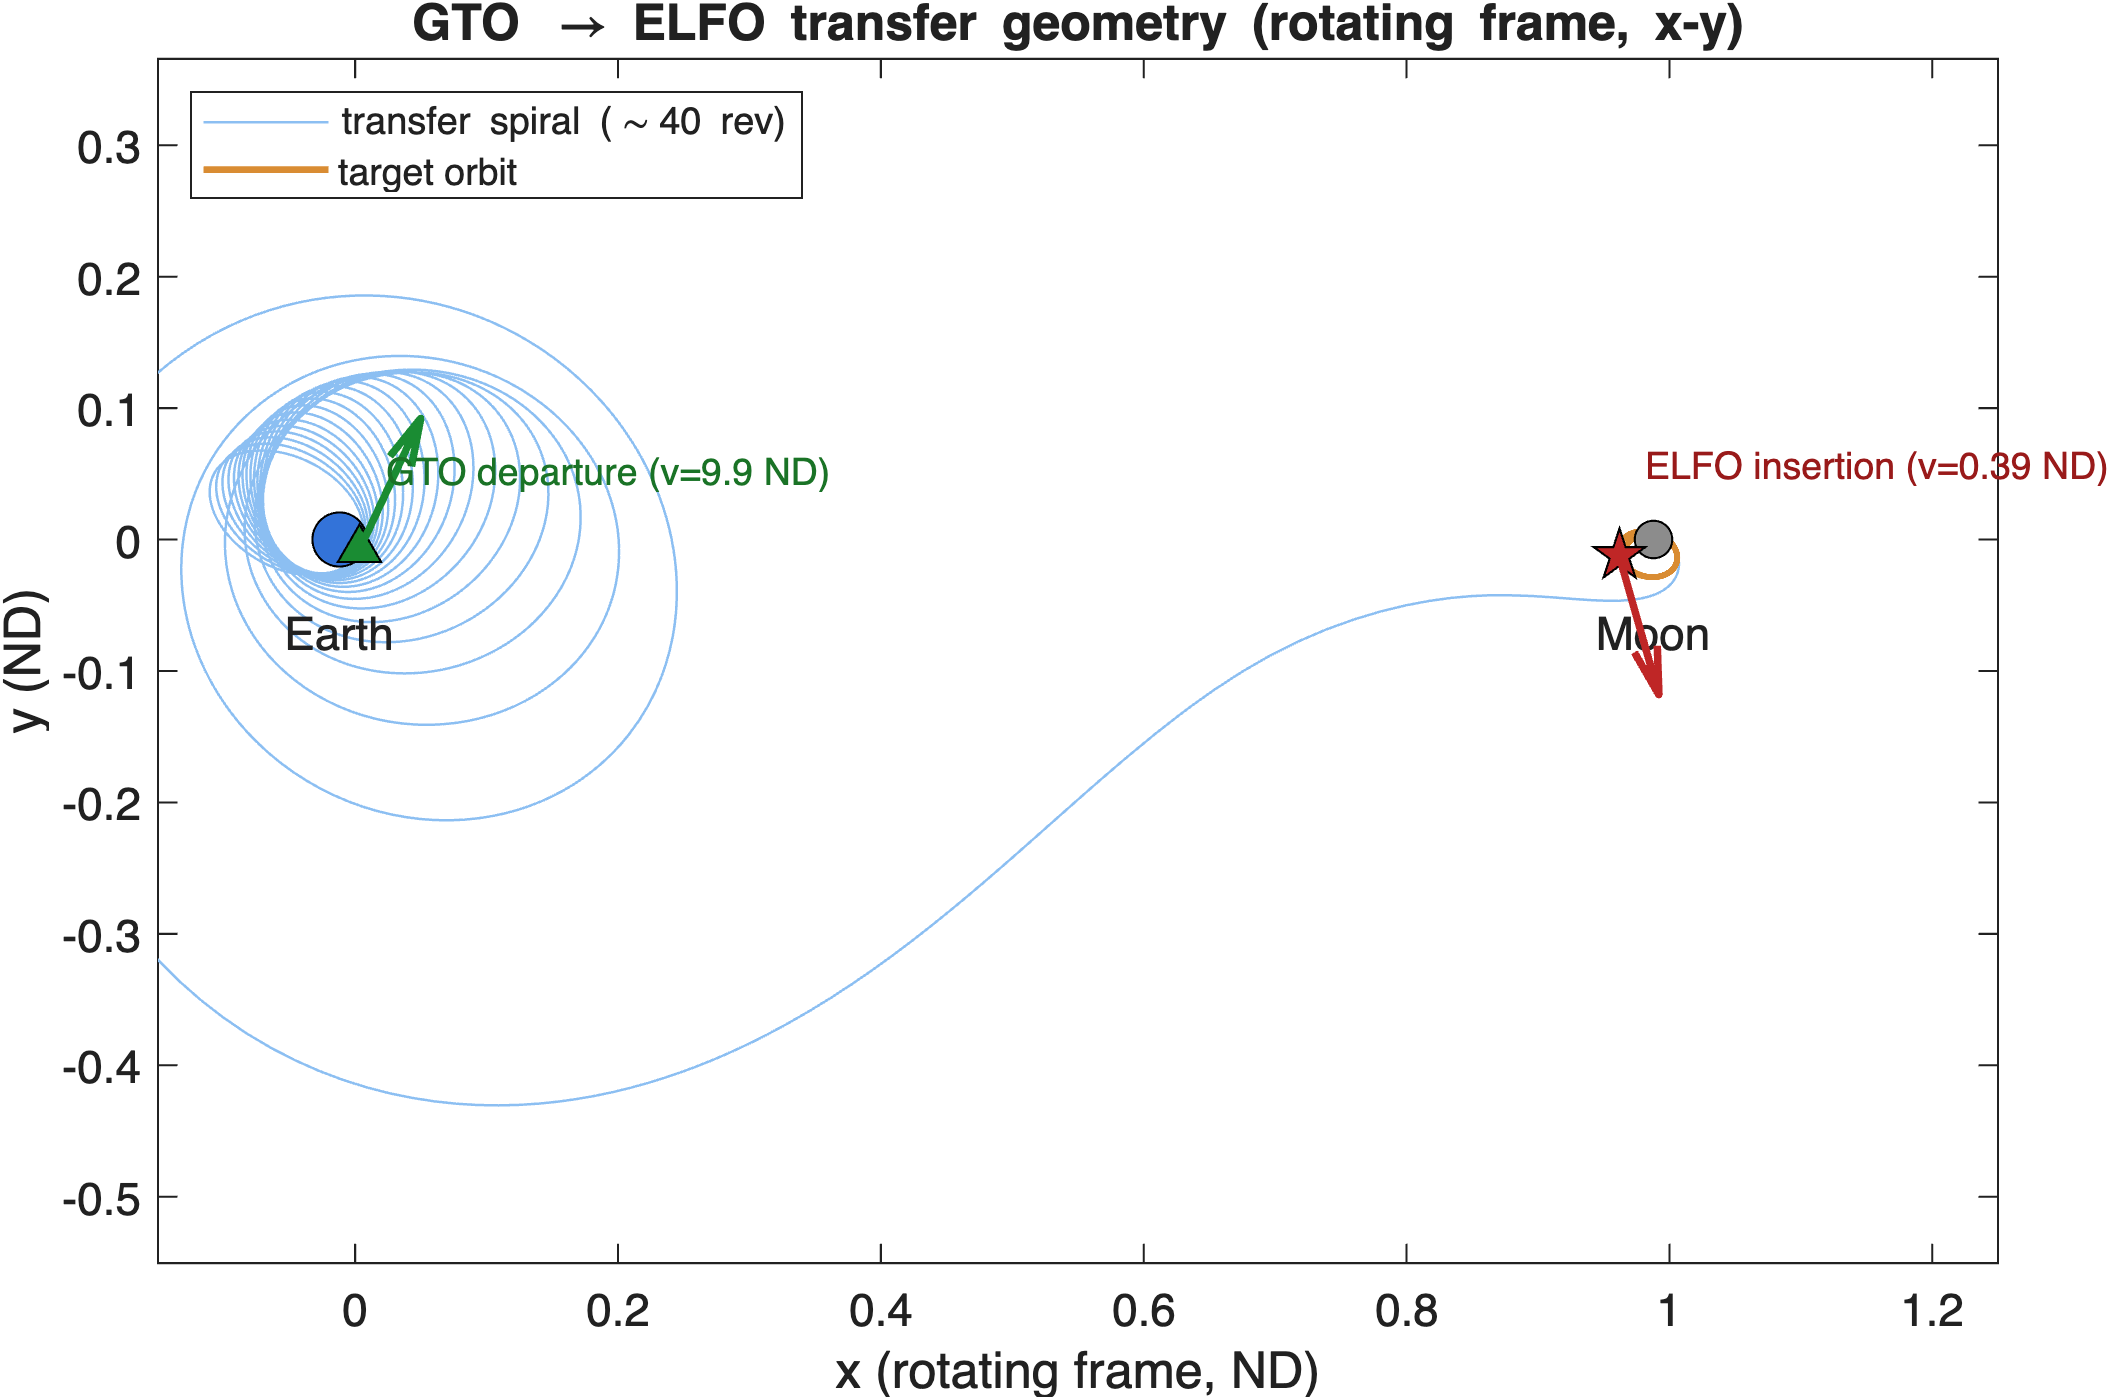
\includegraphics[width=0.82\textwidth]{figures/fig_geometry_elfo.png}
  \caption{GTO\,$\rightarrow$\,ELFO transfer geometry in the rotating
    Earth--Moon frame, produced by the gravity-homotopy ladder. As for the
    tulip, the spiral departs GTO (green, ND speed $9.9$) and inserts at the
    nearest ELFO phase (red star, ND speed $0.39$) on the ELFO (orange) about
    the Moon.}
  \label{fig:geom-elfo}
\end{figure}

%==============================================================================
\section{Stage 3 --- The energy$\rightarrow$fuel homotopy}\label{sec:homotopy}
%==============================================================================

\subsection{The Bertrand--\'Ep\'enoy deformation}
With a converged energy seed in hand, deform the objective from energy to fuel by
a continuation parameter $\varepsilon$:
\begin{equation}
  J(\varepsilon) \;=\; \int_0^{t_f}\! s\,\mathrm{d}t
     \;-\; \varepsilon\!\int_0^{t_f}\! s(1-s)\,\mathrm{d}t,
  \qquad \mathrm{d}t = c\,\kappa\,\mathrm{d}\tau .
  \label{eq:homotopy}
\end{equation}
At $\varepsilon=1$, $J=\int s^2\,\mathrm{d}t$ (energy: strictly convex, smooth
ramp, no restoration). At $\varepsilon=0$, $J=\int s\,\mathrm{d}t$ (fuel:
bang-bang, and equal to propellant up to the positive constant $\Tmax/c$, since
$m(t_f)=1-(\Tmax/c)\int s\,\mathrm{d}t$). Sweeping $\varepsilon:1\!\to\!0$,
warm-starting each solve from the last, sharpens the throttle continuously: the
edge fraction climbs $28\%\!\to\!75\%\!\to\!94\%\!\to\!99.6\%$ and the switch
count grows as the coasts near apogee open up. This is the literal realization of
``start smooth, then sharpen'': deform \emph{from} the convex relaxation
\emph{toward} the non-smooth optimum. $\rightarrow$ \file{sundman\_homotopy.m},
\file{gen\_elfo\_minfuel.m}, \file{minfuel\_at\_tf.m}.

\subsection{The two seeding tricks that made it converge}
The homotopy alone is not enough; two seeding disciplines are load-bearing:
\begin{itemize}
  \item \textbf{No-resample seed.} Map a collocation-feasible warm start onto
        \emph{its own} $\tau$-nodes ($\sigma=\tau/\tau_f$, no \code{pchip}
        interpolation onto a uniform mesh). Downsampling a 40-revolution
        oscillatory trajectory leaves an irreducible $\sim\!10^{-2}$ defect that
        pins IPOPT in restoration (a false ``locally infeasible'' exit). Using
        the seed's own nodes makes the only initial infeasibility the small
        time-trap mismatch, which IPOPT closes to $10^{-14}$ in normal mode.
  \item \textbf{A guarded sweep near $\varepsilon=0$.} A coarse step near the
        bang-bang limit breaks the basin ($\inf_{du}\!\to\!10^{10}$); the tail
        uses fine steps with a guard --- a step that does not converge tight is
        \emph{discarded}, never poisoning the warm start or overwriting the best
        result.
\end{itemize}

\subsection{The certified bang-bang solution}
For the headline tulip case ($t_f=1.15\times$), the sweep reaches
$\varepsilon=0$ machine-tight:
\begin{center}
\begin{tabular}{ll}
\toprule
IPOPT status & \code{Solve\_Succeeded} \\
max collocation defect & $2.4\times10^{-14}$ (machine zero) \\
terminal rendezvous error & $0$ \\
switches & $25$ \\
bang-bang node fraction & $99.4\%$ \\
propellant / $\Delta V$ & $2.264$~kg / $3.370$~km/s \\
\bottomrule
\end{tabular}
\end{center}
The propellant is $23\%$ below the certified $3$-switch burn-then-coast
\emph{local} optimum ($2.950$~kg), confirming that the many-switch
burn-near-perigee / coast-near-apogee structure is the genuine global optimum
rather than a numerical artifact.

\begin{figure}[htbp]
  \centering
  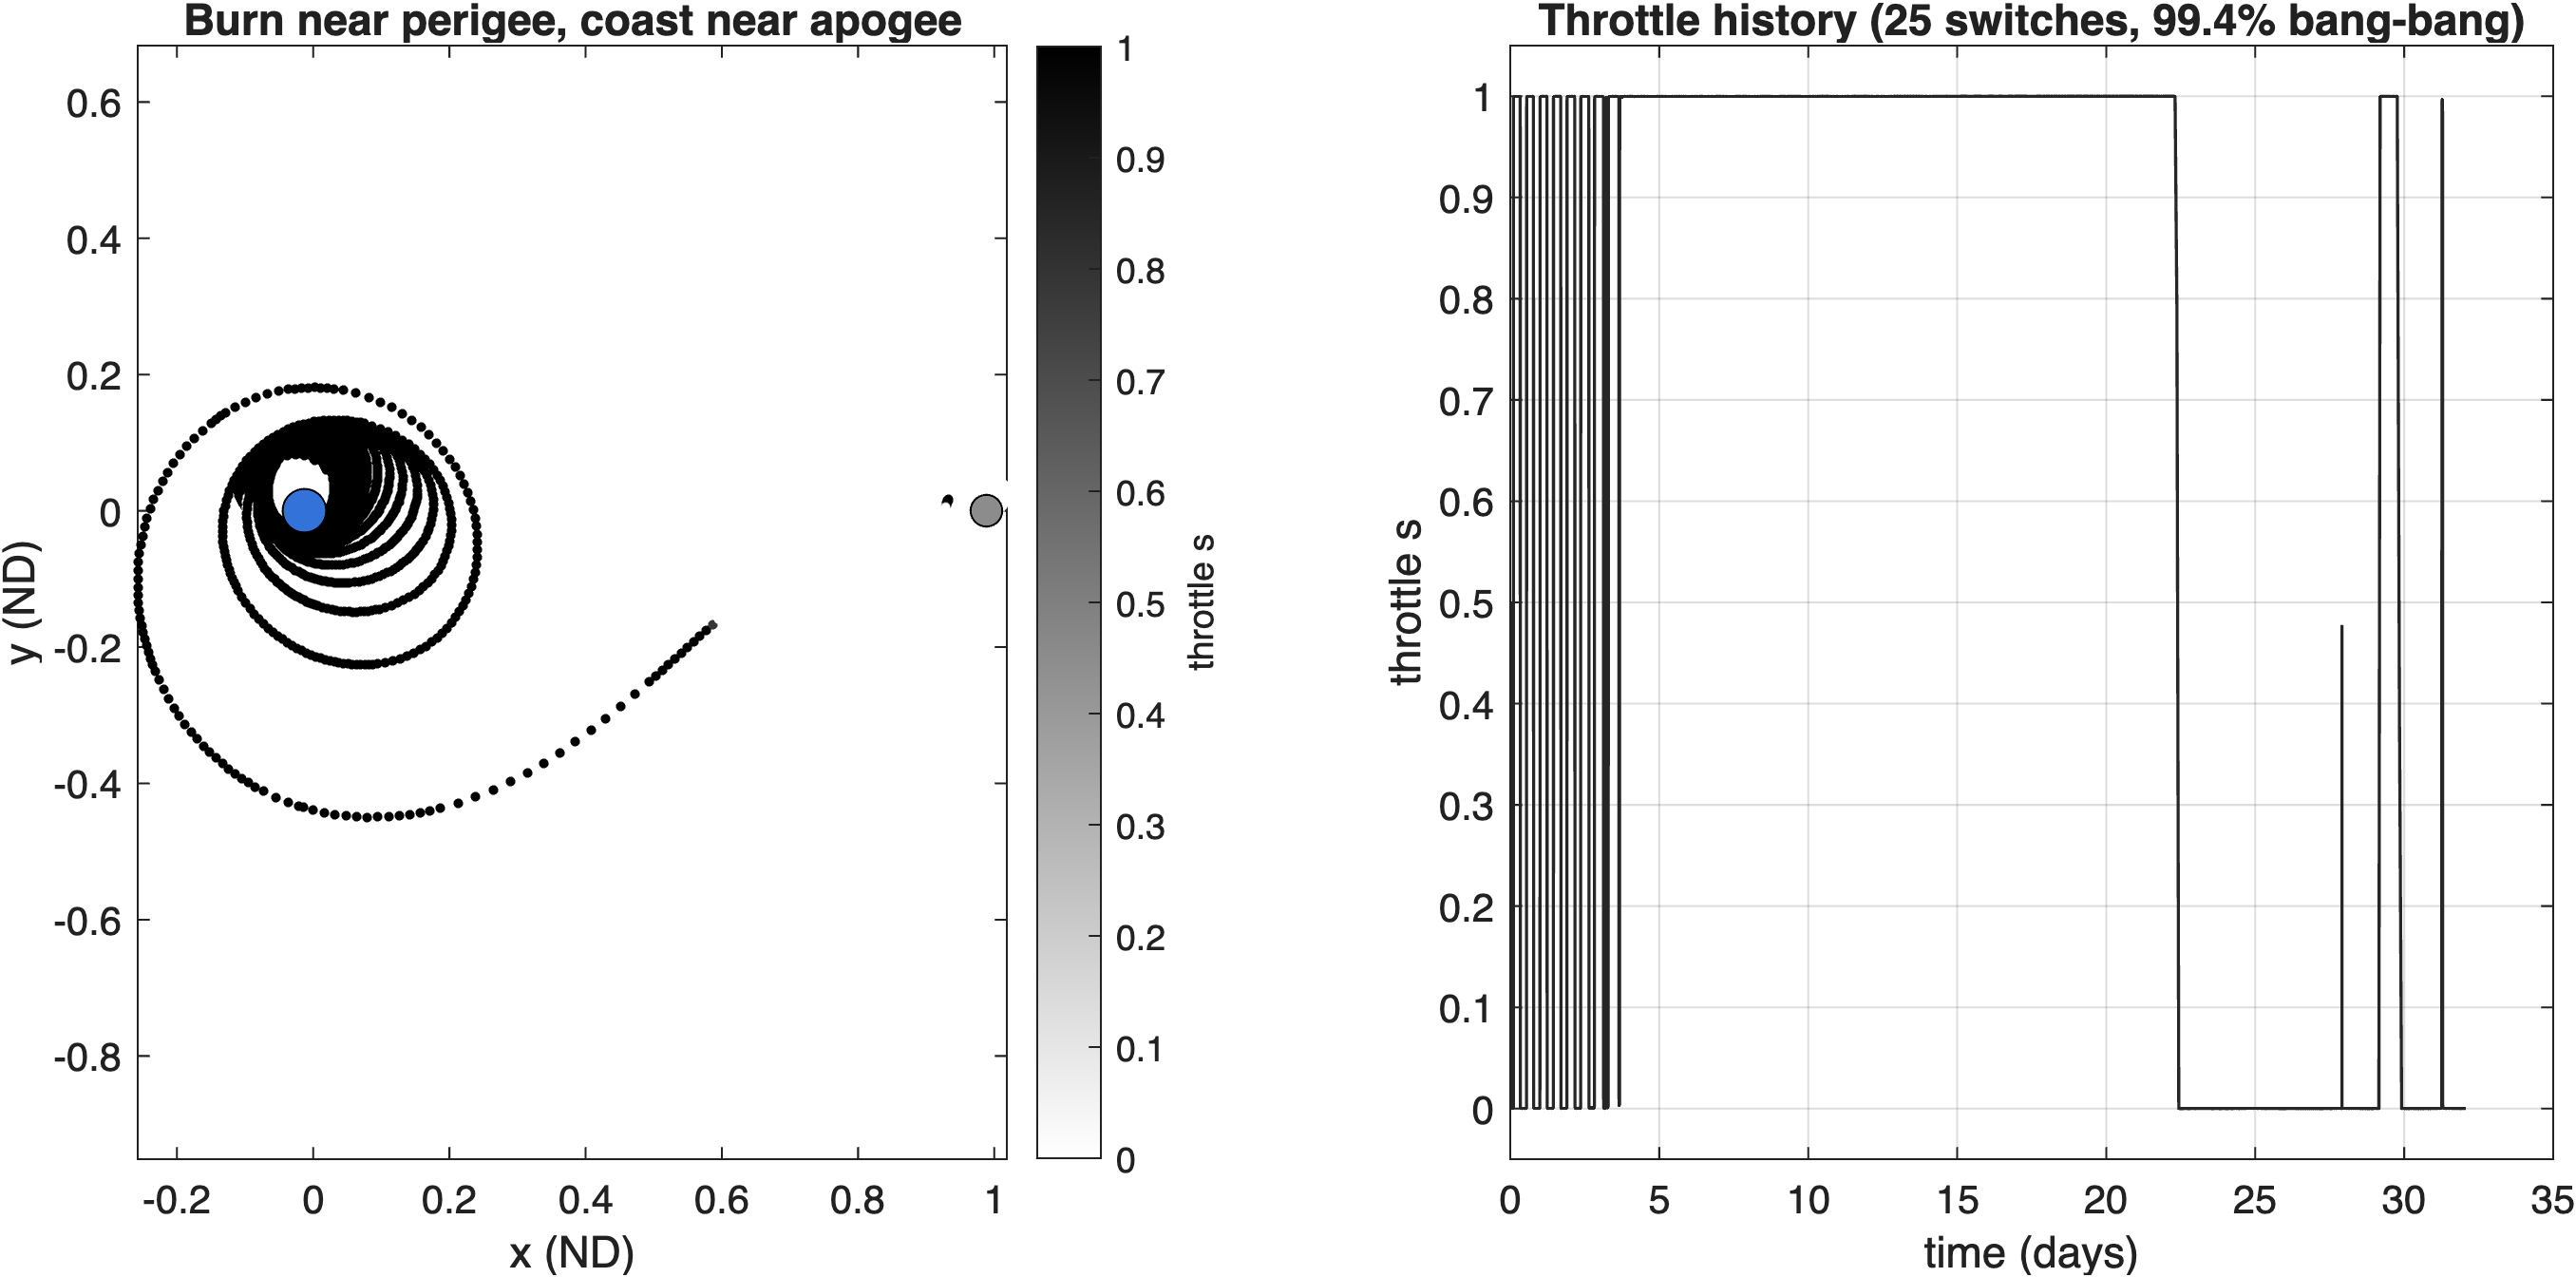
\includegraphics[width=\textwidth]{figures/fig_traj_throttle.png}
  \caption{The certified $\varepsilon=0$ tulip minimum-fuel solution
    ($t_f=1.15\times$). \emph{Left}: the transfer arc colored by throttle
    $s$ --- dense burning near perigee (dark), coasting near apogee (light).
    \emph{Right}: the throttle history is genuinely bang-bang ($99.4\%$ of
    nodes at a bound) with $25$ switches, the sharp early switching giving way
    to a long single burn as the spiral expands.}
  \label{fig:traj-throttle}
\end{figure}

%==============================================================================
\section{Optimality verification}\label{sec:verify}
%==============================================================================
A direct-collocation solution is a KKT point of a \emph{discrete} NLP; it does
not automatically carry a continuous-time optimality certificate. We check it
several independent ways, and we are careful about what each check does and does
not establish.

\subsection{Costates from the KKT duals}
The Lagrange multipliers of the dynamics-defect constraints \eqref{eq:trap} are
the \emph{discrete adjoint} --- the costates $(\boldsymbol\lambda_r,
\boldsymbol\lambda_v,\lambda_m,\lambda_t)$ per interval --- but only \emph{up to
a positive mesh-weight scaling and a global sign}. They are read directly from
the solver (\code{out.lamDef}), avoiding any ill-posed reconstruction from the
primal. Two classes of check follow.

\paragraph{Scale-invariant indicators (strong, calibration-free).} The
primer-vector direction law \eqref{eq:primer} and the transversality condition
are invariant to the unknown positive scaling, so they can be tested without
de-scaling:
\begin{itemize}
  \item \emph{Primer alignment}: the NLP thrust direction matches the costate
        primer $-\boldsymbol\lambda_v/\lVert\boldsymbol\lambda_v\rVert$ to
        $0.06^\circ$--$0.19^\circ$ on every burn arc --- a direct-method solution
        that never forms costates satisfies the PMP direction law to a hundredth
        of a degree.
  \item \emph{Transversality}: $\lambda_m(\tau_f)\approx0$ (free final mass),
        tested \emph{relative} to the costate scale
        ($|\lambda_m(\tau_f)|/\max|\lambda_m|\sim10^{-4}$), since an absolute
        gate would be scale-dependent.
\end{itemize}

\paragraph{Scale-dependent law (requires care).} The switching-function sign law
--- $S<0$ on burns, $S>0$ on coasts, zero-crossings at the switches --- is
\emph{not} scale-invariant (it mixes the unit ``$1$'' with the scaled
$\lVert\boldsymbol\lambda_v\rVert$ and $\lambda_m$ terms of
\eqref{eq:switch}). It requires either de-scaling the duals to node costates or
an empirical single-parameter fit; a na\"ive per-interval reading can misreport
the sign. We flag this honestly: the primer/transversality indicators are
strong, but the switching-law certification is a separate, more delicate step.

\subsection{The independent adjoint-ODE verifier}
The stronger, shooting-free certificate propagates \emph{each burn/coast arc}
forward under the Pontryagin EOM (the regularized 16-dimensional costate
dynamics) from the dual-mapped initial costates, and checks per-arc state
consistency, the Hamiltonian/transversality conditions, and the switch structure
--- with no Levenberg--Marquardt or shooting anywhere. It certifies a direct
bang-bang solution as \emph{consistent with a continuous PMP extremal at the
transcription's $O(h^2)$ resolution}. $\rightarrow$ \file{verify\_direct\_pmp.m}.

\subsection{Model-independent checks}
Two checks need no costates at all and are, in practice, the most trustworthy:
\begin{itemize}
  \item \emph{Solver-free defect recompute}: re-integrate the saved trajectory
        in plain MATLAB (full gravity, the same clock) and recompute the defect
        and rendezvous residual independently of CasADi --- machine zero
        ($\sim10^{-15}$) confirms the discrete solution is genuine.
        $\rightarrow$ \file{verify\_elfo\_seed.m}.
  \item \emph{Mesh-invariance and cross-checks}: the min-time value is identical
        (six figures) from two independent meshes; the $25$-switch $\Delta V$
        matches an earlier uncertified $\sim\!50$-switch estimate to four
        figures. These physical cross-checks, not any single costate test, are
        the real validation.
\end{itemize}

\medskip\noindent\emph{Summary of what is established.} ``Certified'' in this
note means: a machine-tight KKT point of the discrete NLP, PMP-consistent by the
scale-invariant primer and transversality indicators and by the independent
adjoint-ODE verifier, and corroborated by mesh-invariance and propellant/$\Delta
V$ cross-checks. It is \emph{not} a closed continuous-time first-order
certificate (which would require the full de-scaled switching law), and switch
counts/locations are mesh-dependent at trapezoidal $O(h^2)$.

%==============================================================================
\section{The $\Delta V$--time fronts}\label{sec:fronts}
%==============================================================================
Repeating stages 2--3 across a grid of $t_f$ maps the propellant--trip-time
trade for each target.
\begin{itemize}
  \item \textbf{Tulip.} A dense set of \emph{local} minima: with $\sim$40 apogees
        there are combinatorially many near-optimal choices of which to coast
        through, so single-thread continuation lands in whatever basin it drifts
        into and $\Delta V$ scatters. The lower envelope is the real trade ---
        min-time $4.47\to\sim3.0\to2.43$~km/s (campaign-best $2.434$ at
        $1.65\times$, $\sim$46~d, $\sim45\%$ below min-time). First-order PMP
        certification (the switching law of Section~\ref{sec:verify}) holds on
        the band $1.12$--$1.25\times$; higher-$t_f$ points are well-reproduced
        \emph{feasible-envelope} bounds, deliberately distinguished from
        first-order-certified.
  \item \textbf{ELFO.} A cleaner front: monotone $3.344$~km/s ($1.11\times$,
        $31$~d) down to a minimum $2.693$~km/s ($1.73\times$, $48$~d), then flat.
        The optimum sits at a fold, where the many-switch bang-bang is hardest to
        resolve. Of a $14$-factor grid, $11$ reach $\varepsilon=0$ machine-tight
        (edge $\sim99.6\%$).
\end{itemize}
The lower envelope of both fronts --- not the scattered individual solves --- is
the deliverable; pinning the exact envelope needs multi-start per $t_f$.

\begin{figure}[htbp]
  \centering
  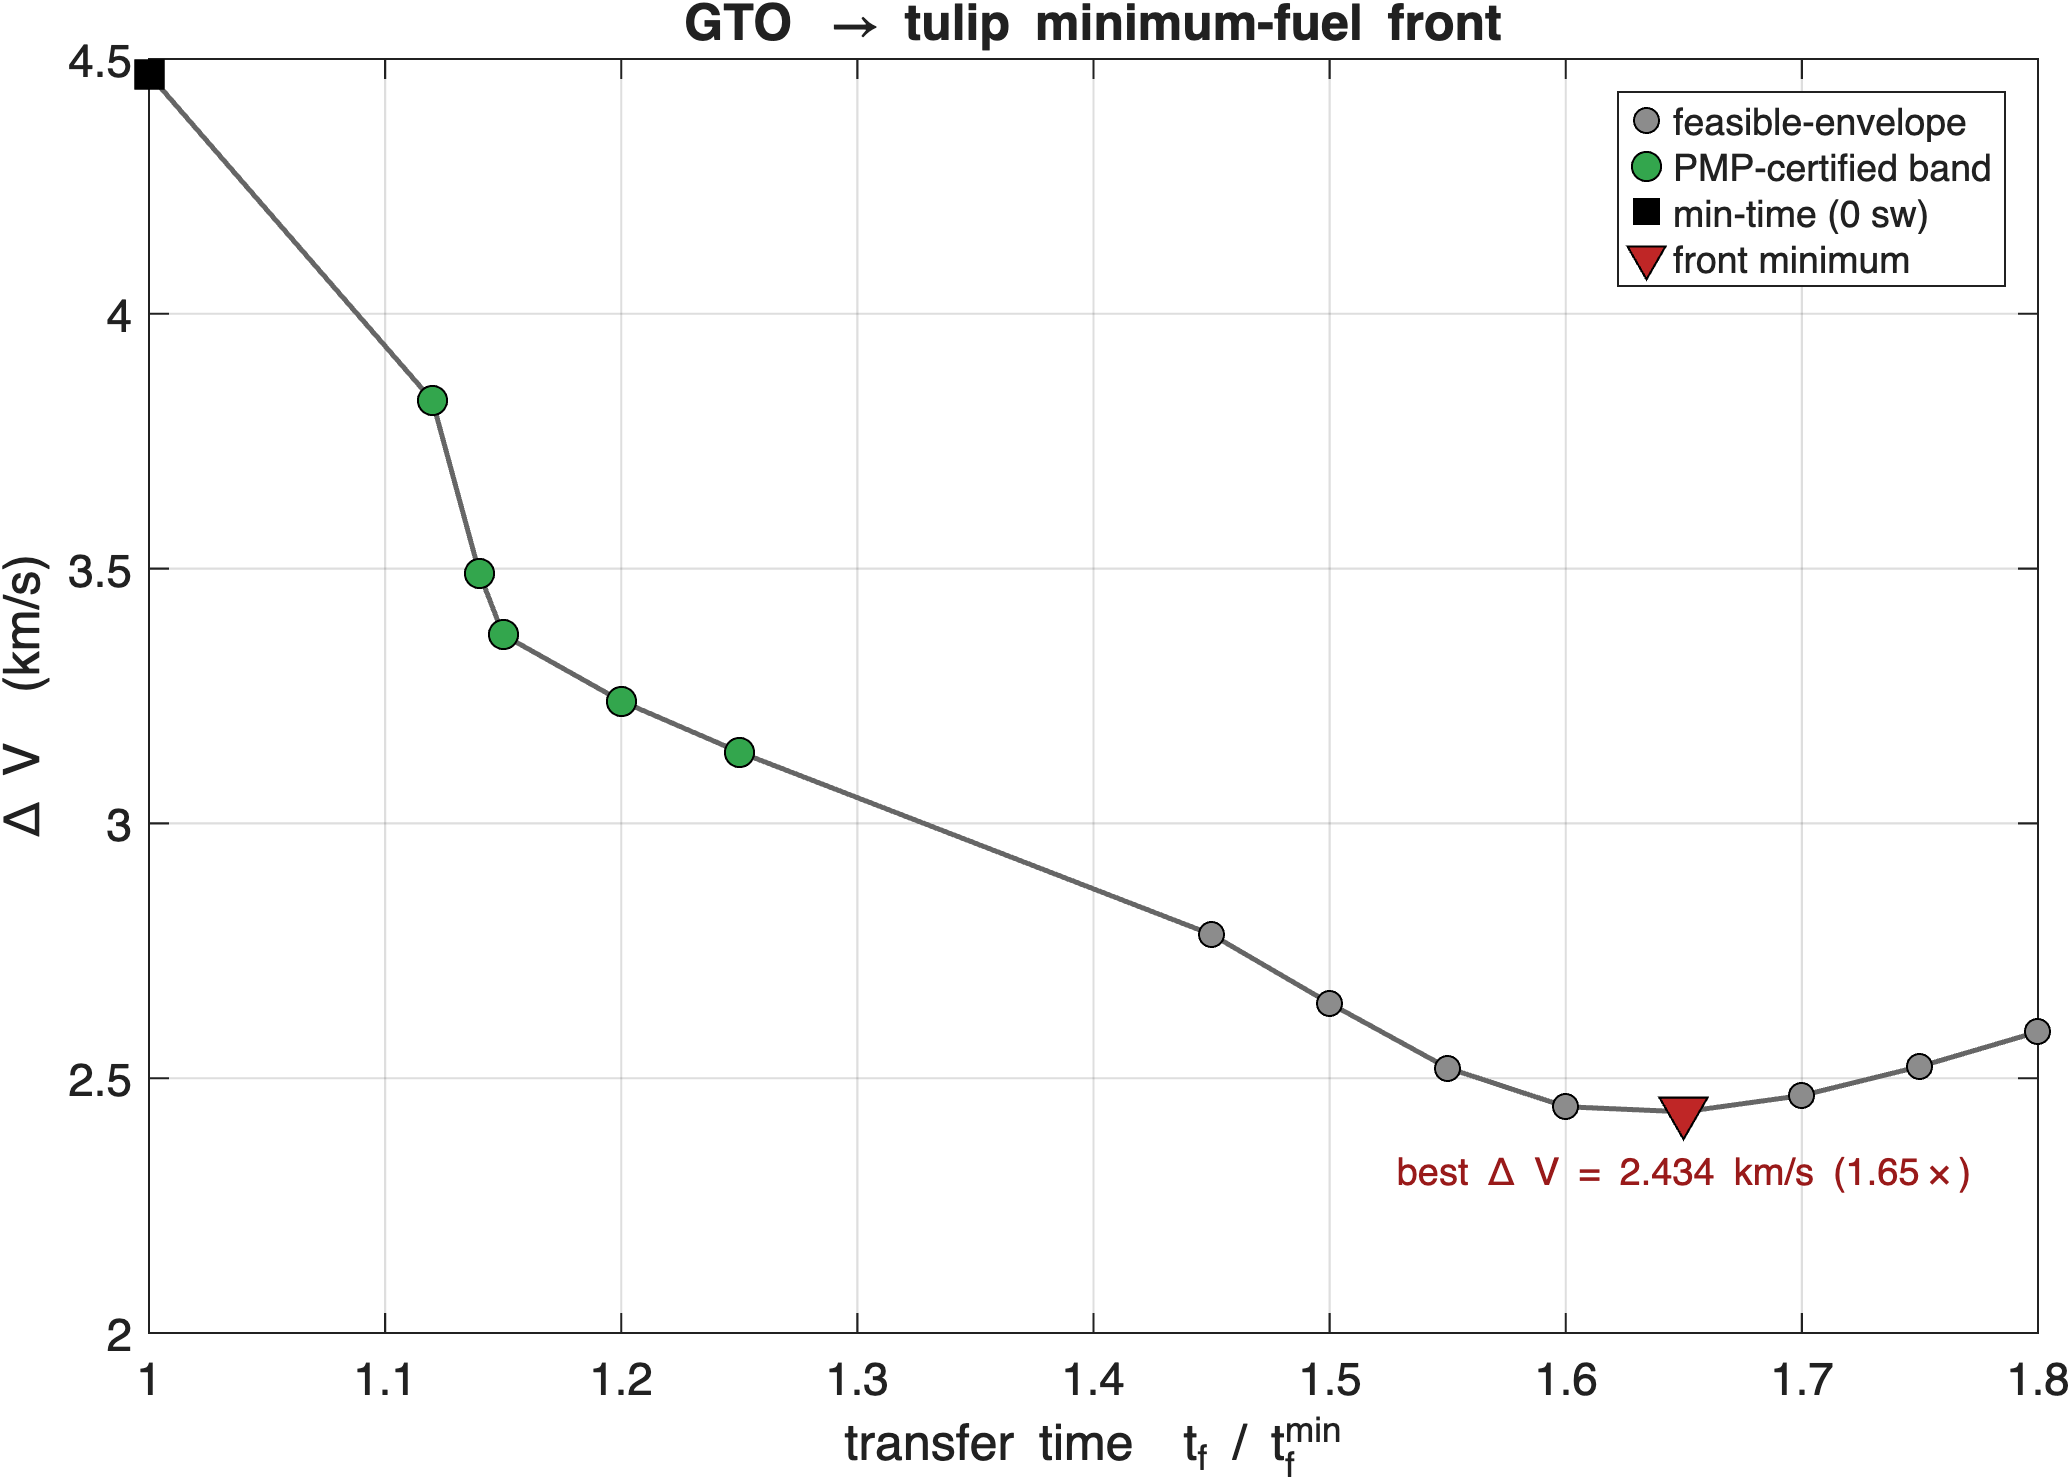
\includegraphics[width=0.49\textwidth]{figures/fig_front_tulip.png}
  \hfill
  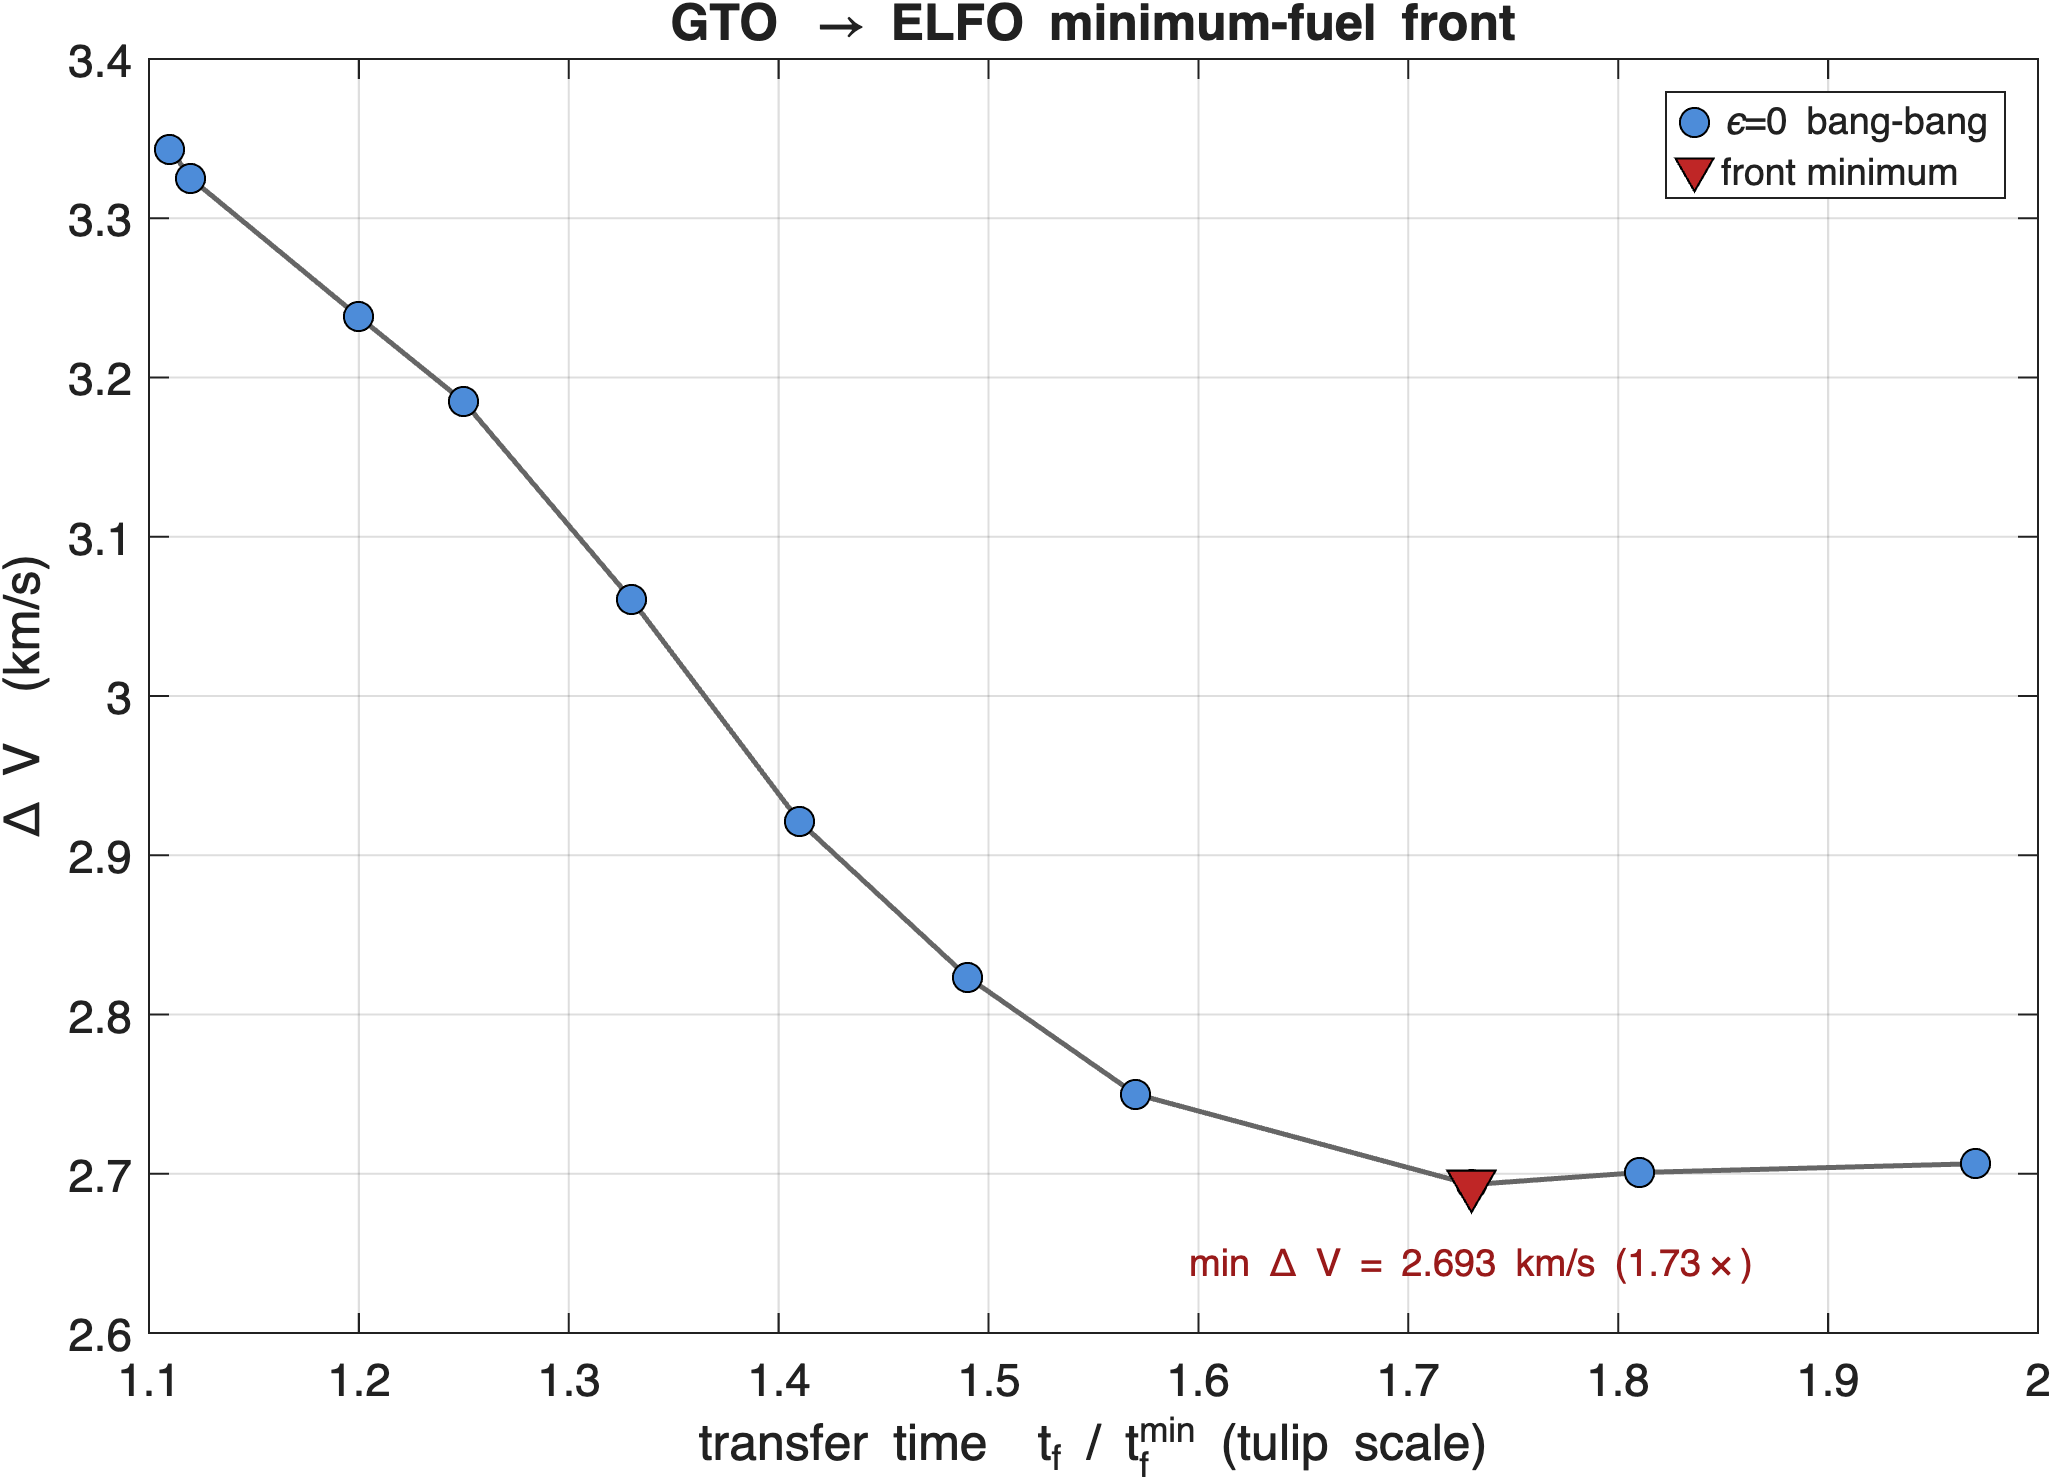
\includegraphics[width=0.49\textwidth]{figures/fig_front_elfo.png}
  \caption{Minimum-fuel $\Delta V$--transfer-time fronts. \emph{Left}: tulip.
    The black square is the $0$-switch min-time endpoint; green points are the
    PMP first-order-certified band ($1.12$--$1.25\times$); grey points are
    well-reproduced feasible-envelope bounds; the front minimum is
    $2.434$~km/s at $1.65\times$ ($\sim46$~d). \emph{Right}: ELFO --- a cleaner,
    near-monotone front reaching a minimum $2.693$~km/s at $1.73\times$
    ($48$~d) before flattening at the fold. Both axes normalize by each
    target's own $t_f^{\min}$ (the ELFO grid retains the tulip-scale abscissa
    of the batch record).}
  \label{fig:fronts}
\end{figure}

%==============================================================================
\section{Lessons learned}\label{sec:lessons}
%==============================================================================
The reusable lessons, several of which cost the most effort:
\begin{enumerate}
  \item \textbf{Two independent walls, dismantled separately.} Objective-side
        (bang-bang non-smoothness) and dynamics-side (the $\sim$40-perigee
        sensitivity + gravitational curvature). Minimum-fuel is hard because it
        hands you both at once; the homotopy removes the first, the Sundman
        regularization the second.
  \item \textbf{Smooth control is the homotopy root.} Minimum-energy is the
        convex relaxation of minimum-fuel; solving it first and deforming toward
        the non-smooth problem is by far the most effective single move. Start
        smooth, then sharpen.
  \item \textbf{Regularize \emph{before} trusting the exact Hessian.} The exact
        NLP Hessian --- an asset for a well-scaled problem --- \emph{destabilizes}
        near the $1/r$ singularities. Sundman lowers the singular exponent by $p$
        \eqref{eq:hessian-scaling} but does not remove it, so (i) a Moon-vicinity
        target needs the \emph{two-primary} clock or the exact Hessian overflows
        (a deterministic MUMPS crash), and (ii) a limited-memory Hessian is the
        safe fallback during continuation --- though it under-solves, so finish
        on the exact Hessian once regularized. Ironically, on the un-regularized
        problem the crude L-BFGS Hessian was \emph{more} stable than the exact one
        precisely because it is damped.
  \item \textbf{The near-min-time wall is fundamental, not a switch-count
        artifact.} As $t_f\to t_f^{\min}$ the throttle saturates, the control
        leaves the interior, and even the \emph{smooth, strictly-convex} energy
        continuation collapses. The transition band ($\sim1.01$--$1.11\times$)
        resists direct \emph{and} indirect methods alike --- a genuine structural
        feature of the problem.
  \item \textbf{Continue from the least-saturated member.} Edge is non-monotone
        in $t_f$; a parameter/target homotopy deforms cleanly only from a
        low-edge root. Check edge before picking the continuation seed.
  \item \textbf{Seed discipline.} No-resample the warm start onto its own nodes
        (interpolation leaves a restoration-pinning defect); loose-continue then
        tight-re-clean the multipliers before sharpening; guard the sweep so a
        bad step is discarded, not propagated.
  \item \textbf{Single shooting is the wrong tool for 40 revolutions.} The
        $\sim\!10^6$ perigee-product sensitivity shrinks the indirect basin to
        nothing for any objective; multiple shooting (or the direct method here)
        is required. Direct collocation with the two regularizations is what
        finally solved the sharp many-switch case.
  \item \textbf{Endpoints must be explicit.} The insertion phase is a modeling
        choice that materially changes the transfer; threading it implicitly from
        seed files let it drift silently. Declaring $\rv_0,\rv_f$ in one source of
        truth, guarded, is the structural fix (Appendix~A).
\end{enumerate}

%==============================================================================
\section*{Appendix A --- Code map}\label{sec:code-endpoints}
\addcontentsline{toc}{section}{Appendix A --- Code map}
%==============================================================================
\noindent The pipeline is a self-contained set of MATLAB/CasADi modules under
\file{NLP\_lowThrust\_GTO\_tulip/}:
\begin{itemize}\itemsep1pt
  \item \textbf{Core solvers} --- \file{sundman\_minfuel/casadi\_minfuel\_sundman.m}
        (fixed-$t_f$, single-primary; the original), \file{elfo/casadi\_energy\_freetf.m}
        (free-$t_f$ slack, two-primary clock, energy$\to$fuel objective),
        \file{elfo/casadi\_mintime\_freetf.m} (all-burn min-time sibling).
  \item \textbf{Endpoints (single source of truth)} --- the helper
        \file{insertion\_states.m} returns \code{[rv0, rvf, meta]} for a given
        \code{target} (\code{'tulip'} or \code{'elfo'}) and a named
        \code{criterion} --- tulip \code{'campaign'}, \code{'maxydot'},
        \code{'apoapsis'}; ELFO \code{'nearest'}, \code{'apolune'},
        \code{'perilune'}. Every driver declares its endpoints through it and
        asserts the loaded seed matches (a fail-loud drift guard); every output
        records \code{rv0}, \code{rvf}, and the \code{insertion} label.
  \item \textbf{Stage drivers} --- min-time
        \file{gen\_tulip\_mintime.m} / \file{gen\_elfo\_mintime.m};
        energy seeds \file{gen\_energy\_seed.m}, \file{gen\_tulip\_energy\_2p.m},
        \file{gen\_elfo\_energy\_gravhom.m}, and
        \file{gen\_elfo\_energy\_tfsweep.m};
        fuel homotopy \file{sundman\_homotopy.m}, \file{gen\_elfo\_minfuel.m},
        and \file{minfuel\_at\_tf.m}.
  \item \textbf{Verification} --- \file{verify\_direct\_pmp.m} (adjoint-ODE),
        \file{verify\_elfo\_seed.m} (solver-free defect).
\end{itemize}

\paragraph{Fixed constants (ND).} $\muS=0.012150585609624$; $\Tmax$ and $c$
from $25$~mN, $15$~kg, $I_{sp}=2100$~s; endpoints
\begin{align*}
  \rv_0 &= (0.003496,\,-0.007296,\,0,\ 4.1915,\,8.9887,\,0)
          &&\text{(GTO departure)},\\
  \rv_f &= (1.00658,\,0.04257,\,-0.05578,\ -0.16004,\,0.06657,\,-0.26046)
          &&\text{(tulip \code{campaign})}.
\end{align*}

\paragraph{External review.} The three core solvers and the homotopy/seed recipe
were reviewed (2026-07-15) by GPT-5.6-terra and Gemini~3.1~Pro: the physics,
Sundman scaling, two-primary asymptotes, homotopy measure, CR3BP signs, and
trapezoidal defects were confirmed correct; the review's precision points (the
Hessian scaling \eqref{eq:hessian-scaling}, the all-burn labeling of
\eqref{eq:mintime}, the pinned-$t_f$ nature of the energy ladder, and the
scale-invariant-indicator framing of Section~\ref{sec:verify}) are incorporated
above. Full triage in \file{doc/reviews/}.

\end{document}
